\documentclass[12pt,a4paper,oneside,brazil,chapter=TITLE,section=TITLE]{abntex2}

\usepackage[T1]{fontenc}
\usepackage[utf8]{inputenc}
\usepackage[brazil]{babel}
\usepackage{lmodern}
\usepackage{microtype}
\usepackage{graphicx}
\usepackage{amsmath,amssymb}
\usepackage{booktabs}
\usepackage{float}
\usepackage{listings}
\usepackage{xcolor}
\usepackage{caption}
\usepackage{subcaption}
\usepackage{geometry}
\usepackage{abntex2cite}
\usepackage{url}

\geometry{top=3cm,bottom=2cm,left=3cm,right=2cm}

\lstset{
  basicstyle=\ttfamily\footnotesize,
  breaklines=true,
  keywordstyle=\color{blue!70!black}\bfseries,
  commentstyle=\color{green!50!black}\itshape,
  stringstyle=\color{red!60!black},
  numbers=left, numberstyle=\tiny\color{gray},
  numbersep=6pt, frame=single, rulecolor=\color{gray!40},
  tabsize=2, showstringspaces=false,
}
\lstdefinestyle{matlab}{language=Matlab}

\titulo{Projeto 7 -- Segmenta\c{c}\~ao: Fronteiras dos Dois Maiores Blobs}
\autor{Matheus Serr\~ao Uch\^oa}
\local{Manaus -- AM}
\data{maio de 2026}
\instituicao{%
  Universidade Federal do Amazonas -- UFAM\\
  Instituto de Computa\c{c}\~ao -- IComp\\
  Disciplina: Processamento Digital de Imagens}
\tipotrabalho{Relat\'orio de Atividade}
\preambulo{Relat\'orio referente ao Projeto~7 da disciplina de
  Processamento Digital de Imagens, abordando segmenta\c{c}\~ao por
  limiariza\c{c}\~ao de Otsu e extra\c{c}\~ao das fronteiras dos dois
  maiores blobs em tr\^es imagens.}

\hypersetup{
  colorlinks=true, linkcolor=blue!60!black,
  citecolor=green!50!black, urlcolor=blue
}

\begin{document}

%% ================================================================
\begin{capa}
  \center
  
\includegraphics[width=3cm]{ufam_logo.png}\\[0.5cm]
  {\large\bfseries Universidade Federal do Amazonas}\\
  {\large Instituto de Computa\c{c}\~ao -- IComp}\\[1cm]
  \vfill
  {\LARGE\bfseries Processamento Digital de Imagens}\\[0.4cm]
  {\Large\bfseries Projeto 7}\\[0.3cm]
  {\large Segmenta\c{c}\~ao: Fronteiras dos Dois Maiores Blobs}\\
  \vfill
  {\large Matheus Serr\~ao Uch\^oa}\\[0.5cm]
  {\large Manaus -- AM, maio de 2026}
\end{capa}

\begin{folhaderosto}
  \begin{center}
    {\large\bfseries Matheus Serr\~ao Uch\^oa}\\[2cm]
    {\LARGE\bfseries Projeto 7 -- Segmenta\c{c}\~ao}\\[1.5cm]
  \end{center}
  \begin{flushright}
    \begin{minipage}{9cm}
      \small
      Relat\'orio apresentado como atividade avaliativa da disciplina
      de Processamento Digital de Imagens do Instituto de Computa\c{c}\~ao
      da Universidade Federal do Amazonas.
    \end{minipage}
  \end{flushright}
  \vfill
  \begin{center}{\large Manaus -- AM, maio de 2026}\end{center}
\end{folhaderosto}

\begin{resumo}
Este relat\'orio descreve a segmenta\c{c}\~ao autom\'atica de tr\^es
imagens digitais com o objetivo de extrair as fronteiras dos dois
maiores \textit{blobs} (regi\~oes conectadas) em cada uma delas.
O m\'etodo adotado combina limiariza\c{c}\~ao de Otsu para binariza\c{c}\~ao,
opera\c{c}\~oes morfol\'ogicas de abertura e fechamento para remo\c{c}\~ao
de ru\'ido, rotula\c{c}\~ao de componentes conectados com sele\c{c}\~ao
dos dois maiores e extra\c{c}\~ao de contornos por diferen\c{c}a
morfol\'ogica entre o blob e sua eros\~ao.
Os resultados demonstram que o pipeline proposto isola corretamente os
dois maiores blobs nas tr\^es imagens, com \'areas variando entre 13.386
e 17.100 pixels, e sobrep\~oe os contornos na imagem original para
visualiza\c{c}\~ao.

\vspace{0.5cm}
\noindent\textbf{Palavras-chave:}
Segmenta\c{c}\~ao.
Limiariza\c{c}\~ao de Otsu.
Morfologia matem\'atica.
Componentes conectados.
Detec\c{c}\~ao de fronteiras.
\end{resumo}

\tableofcontents*
\cleardoublepage
\textual

%% ----------------------------------------------------------------
\chapter{Introdu\c{c}\~ao}
%% ----------------------------------------------------------------

A segmenta\c{c}\~ao de imagens \'e uma das etapas fundamentais do
processamento digital de imagens, permitindo separar regi\~oes de
interesse (\textit{blobs}, objetos) do fundo.
Neste projeto, o objetivo \'e extrair automaticamente as
\textbf{fronteiras dos dois maiores blobs} em cada uma das tr\^es
imagens fornecidas (Imagem1.jpg, Imagem2.jpg, Imagem3.jpg).

O m\'etodo escolhido combina t\'ecnicas cl\'assicas bem fundamentadas:
\begin{itemize}
  \item \textbf{Limiariza\c{c}\~ao de Otsu} \cite{otsu1979}: determina
        automaticamente o limiar \'otimo que maximiza a vari\^ancia entre
        classes;
  \item \textbf{Morfologia matem\'atica} \cite{serra1982}: abertura e
        fechamento para limpeza da m\'ascara bin\'aria;
  \item \textbf{Rotula\c{c}\~ao de componentes conectados}
        \cite{rosenfeld1966}: identifica e enumera os blobs;
  \item \textbf{Extra\c{c}\~ao de contorno morfol\'ogico}: fronteira =
        blob $\setminus$ eros\~ao(blob).
\end{itemize}

%% ----------------------------------------------------------------
\chapter{Fundamenta\c{c}\~ao Te\'orica}
%% ----------------------------------------------------------------

\section{Limiariza\c{c}\~ao de Otsu}

O m\'etodo de Otsu \cite{otsu1979} encontra o limiar $T^*$ que maximiza
a vari\^ancia entre classes (\textit{between-class variance}):
\begin{equation}
  T^* = \arg\max_T \; \sigma_B^2(T)
      = \arg\max_T \; \omega_0(T)\,\omega_1(T)\,[\mu_0(T) - \mu_1(T)]^2,
\end{equation}
onde $\omega_k$ s\~ao as probabilidades acumuladas e $\mu_k$ as m\'edias
de cada classe.
A vantagem sobre um limiar fixo \'e que $T^*$ se adapta ao histograma
de cada imagem, sem necessidade de ajuste manual.

\section{Morfologia Matem\'atica}

Para remover ru\'ido da m\'ascara bin\'aria, s\~ao aplicadas:
\begin{itemize}
  \item \textbf{Abertura morfol\'ogica} ($f \circ b = (f \ominus b) \oplus b$):
        elimina pequenos objetos menores que o elemento estruturante $b$;
  \item \textbf{Fechamento morfol\'ogico} ($f \bullet b = (f \oplus b) \ominus b$):
        preenche pequenos buracos dentro dos blobs.
\end{itemize}

\section{Componentes Conectados e Extra\c{c}\~ao de Fronteiras}

A rotula\c{c}\~ao de componentes conectados \cite{rosenfeld1966} associa
um r\'otulo \'unico a cada conjunto de pixels 8-conectados na m\'ascara
bin\'aria. Os dois maiores componentes (por \'area em pixels) s\~ao
retidos.

A fronteira de um blob $B$ \'e extra\'ida por:
\begin{equation}
  \partial B = B \setminus (B \ominus b),
\end{equation}
onde $B \ominus b$ \'e a eros\~ao de $B$ pelo elemento estruturante $b$
(disco de raio 2). O resultado \'e uma borda de espessura $\approx 2$
pixels sobreosta na imagem original.

%% ----------------------------------------------------------------
\chapter{Implementa\c{c}\~ao}
%% ----------------------------------------------------------------

O c\'odigo MATLAB \texttt{main\_project9.m} processa cada imagem
seguindo o pipeline descrito. O trecho central \'e:

\begin{lstlisting}[style=matlab,
  caption={Trecho central do pipeline de segmenta\c{c}\~ao}]
gray  = rgb2gray(rgb);
T     = graythresh(gray);           % Otsu normalizado [0,1]
mask  = imbinarize(gray, T);        % classe minoritaria = blobs

se    = strel('disk', 3);
mask_clean = imopen(mask, se);      % remove pequenos blobs
mask_clean = imclose(mask_clean, se); % fecha buracos

cc     = bwconncomp(mask_clean, 8);
stats  = regionprops(cc, 'Area');
areas  = [stats.Area];
[~, sort_idx] = sort(areas, 'descend');
labeled = labelmatrix(cc);

blob1  = (labeled == sort_idx(1));
blob2  = (labeled == sort_idx(2));

se_e   = strel('disk', 2);
bnd1   = blob1 & ~imerode(blob1, se_e);  % fronteira blob 1
bnd2   = blob2 & ~imerode(blob2, se_e);  % fronteira blob 2
\end{lstlisting}

%% ----------------------------------------------------------------
\chapter{Resultados}
%% ----------------------------------------------------------------

\section{Vis\~ao Geral das Tr\^es Imagens}

A Figura~\ref{fig:summary} apresenta as tr\^es imagens originais (linha
superior) e os respectivos resultados com os contornos dos dois maiores
blobs sobrepostos (linha inferior).

\begin{figure}[H]
  \centering
  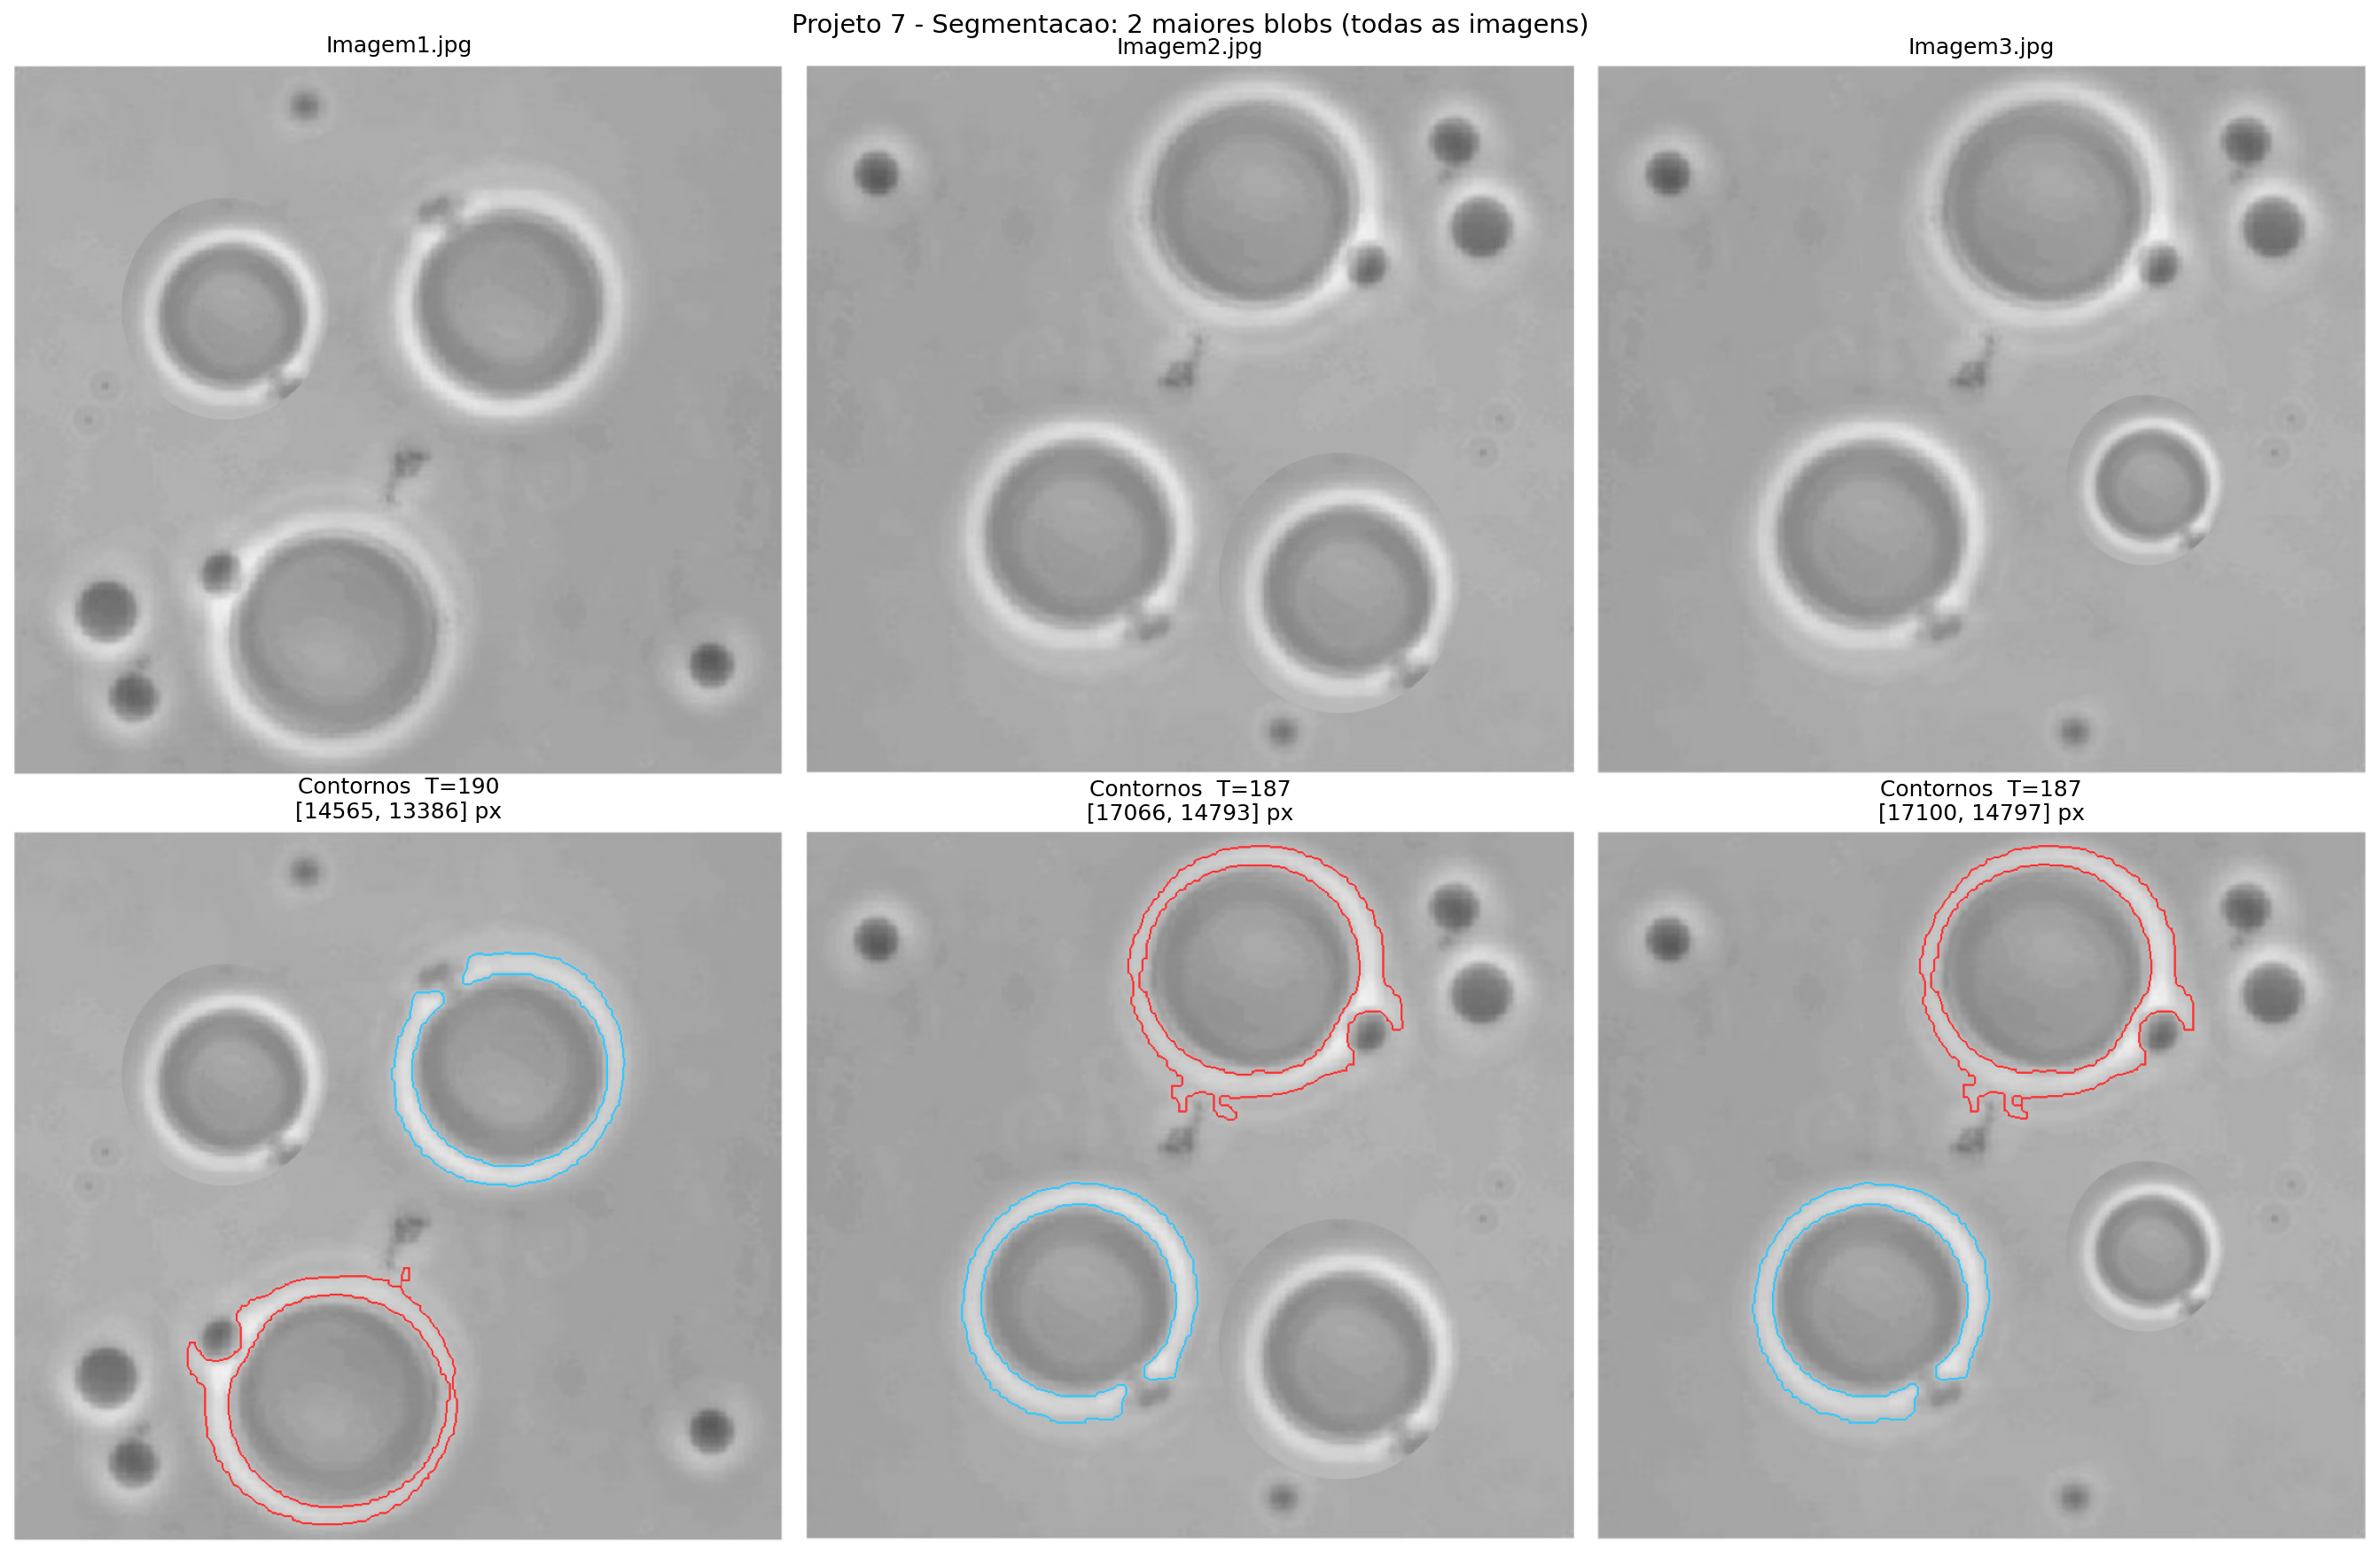
\includegraphics[width=\linewidth]{imgs_result/summary_all.png}
  \caption{Resumo: imagens originais (acima) e contornos dos dois
           maiores blobs sobrepostos (abaixo).
           Contorno vermelho = blob 1 (maior);
           contorno ciano = blob 2.}
  \label{fig:summary}
  \fonte{Elaborado pelo autor (2026).}
\end{figure}

\section{Imagem 1 -- Imagem1.jpg}

\begin{figure}[H]
  \centering
  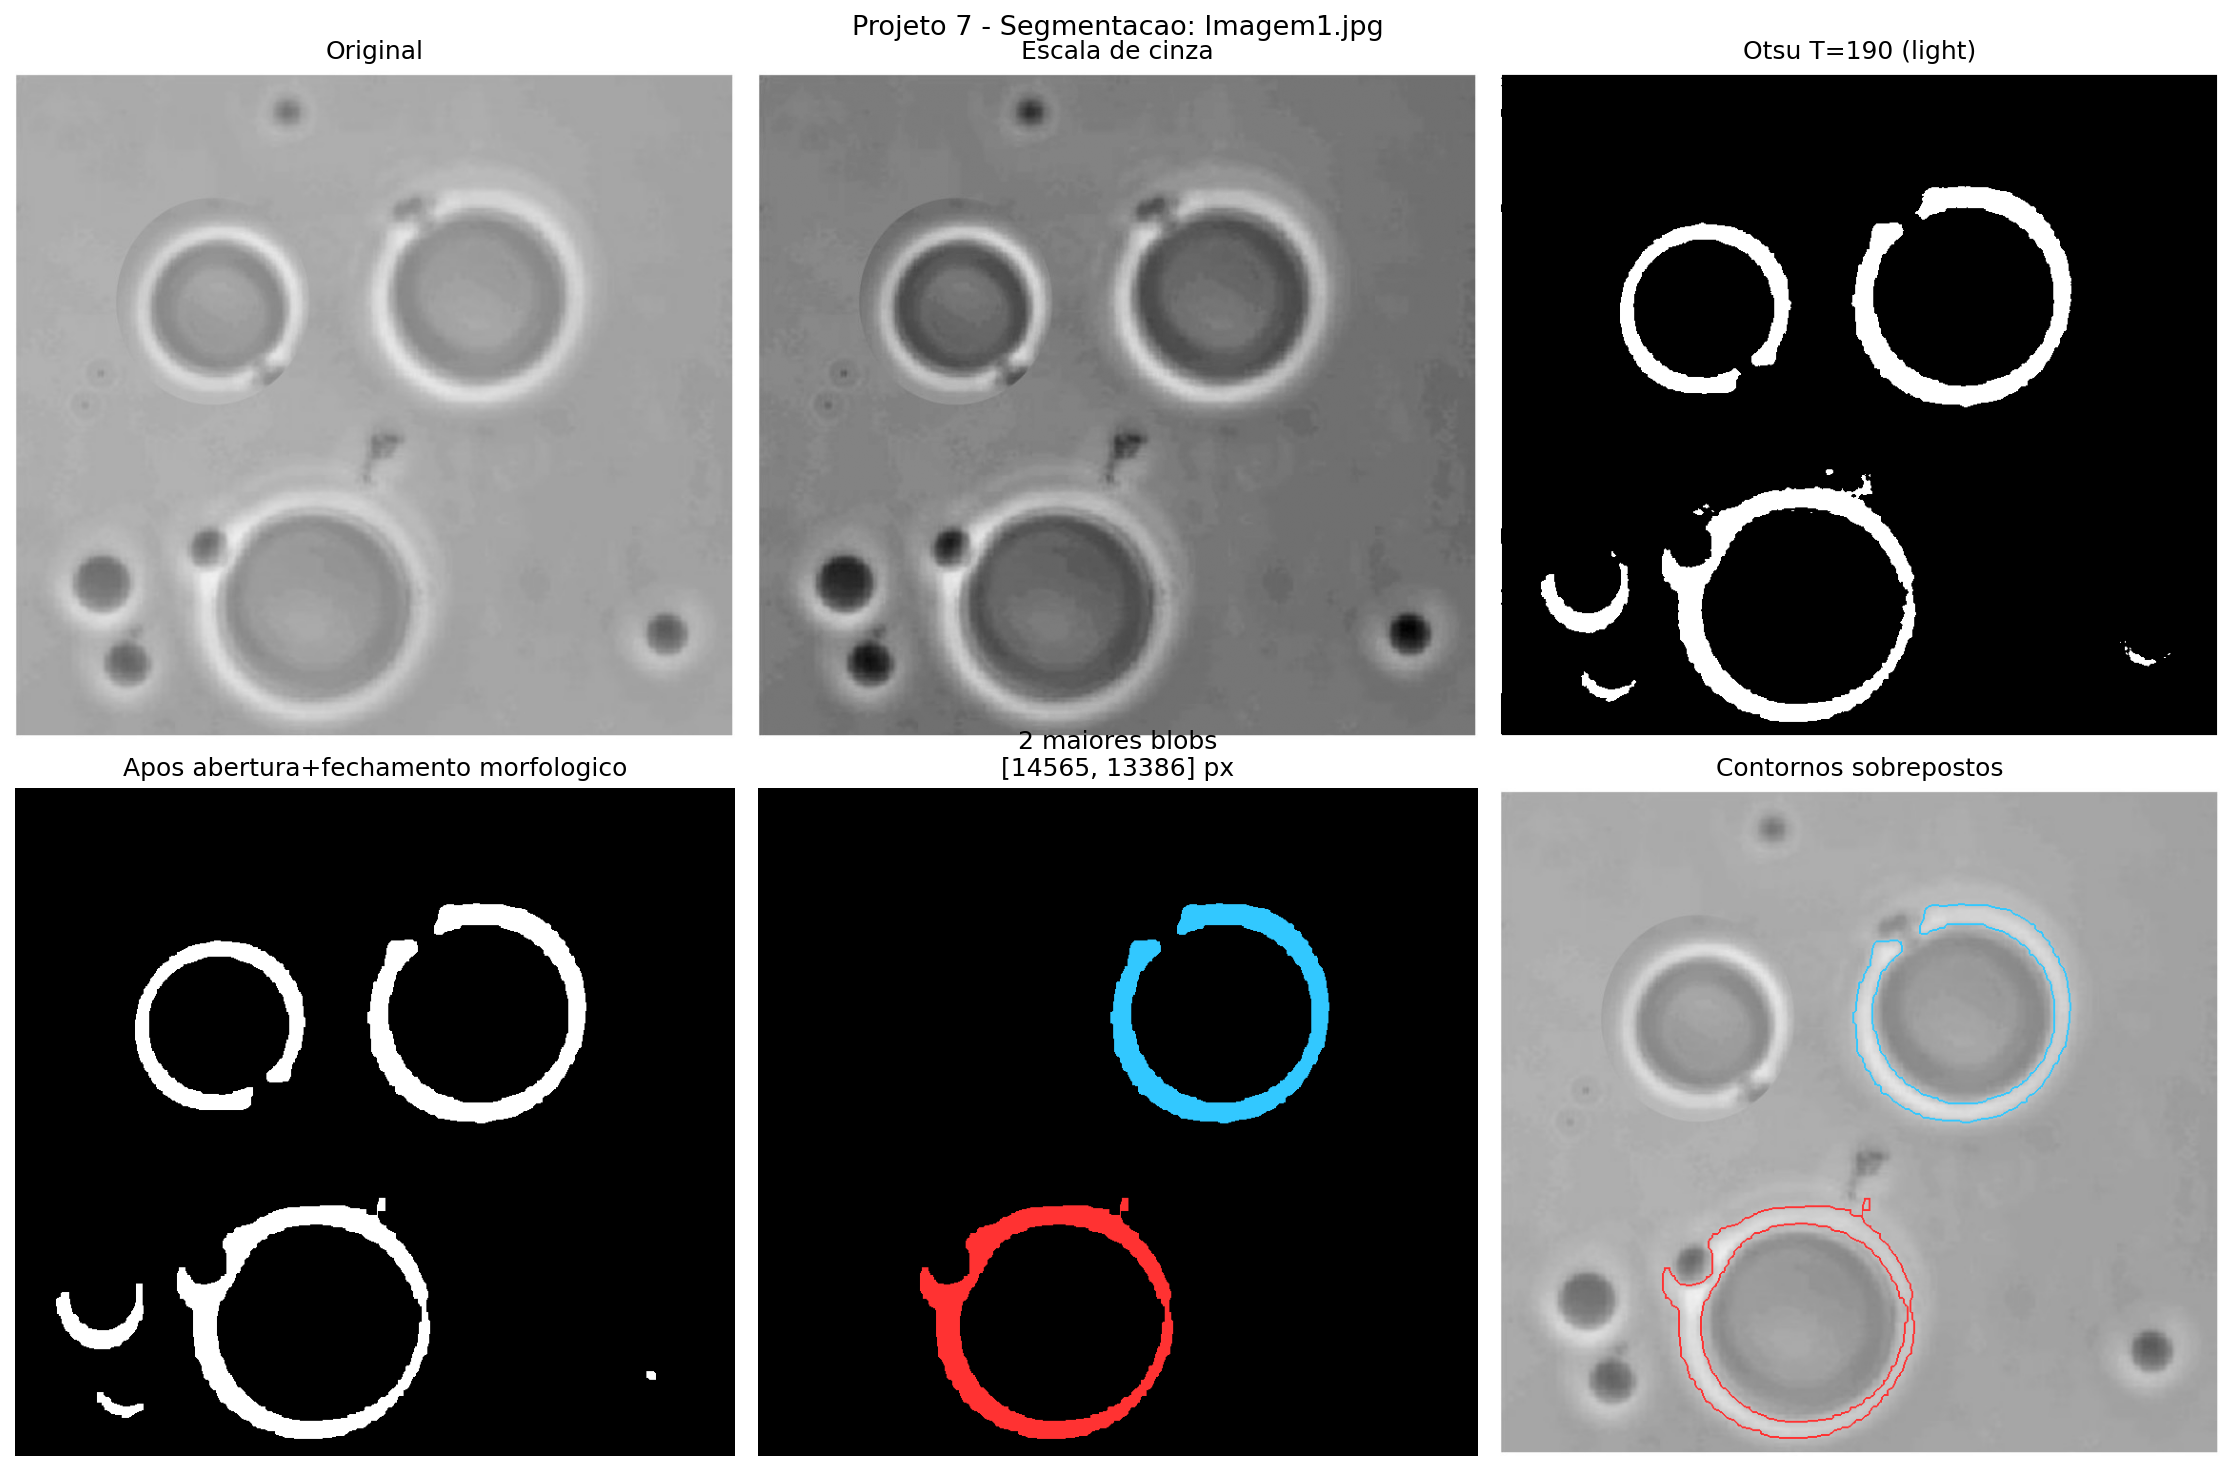
\includegraphics[width=\linewidth]{imgs_result/imagem1_pipeline.png}
  \caption{Pipeline completo para Imagem1.jpg:
           original, escala de cinza, Otsu binarizado,
           m\'ascara ap\'os limpeza, mapa de r\'otulos e
           contornos sobrepostos.
           Limiar Otsu $T = 190$; 6~componentes detectados;
           2~maiores: 14.565 e 13.386 pixels.}
  \fonte{Elaborado pelo autor (2026).}
\end{figure}

\begin{figure}[H]
  \centering
  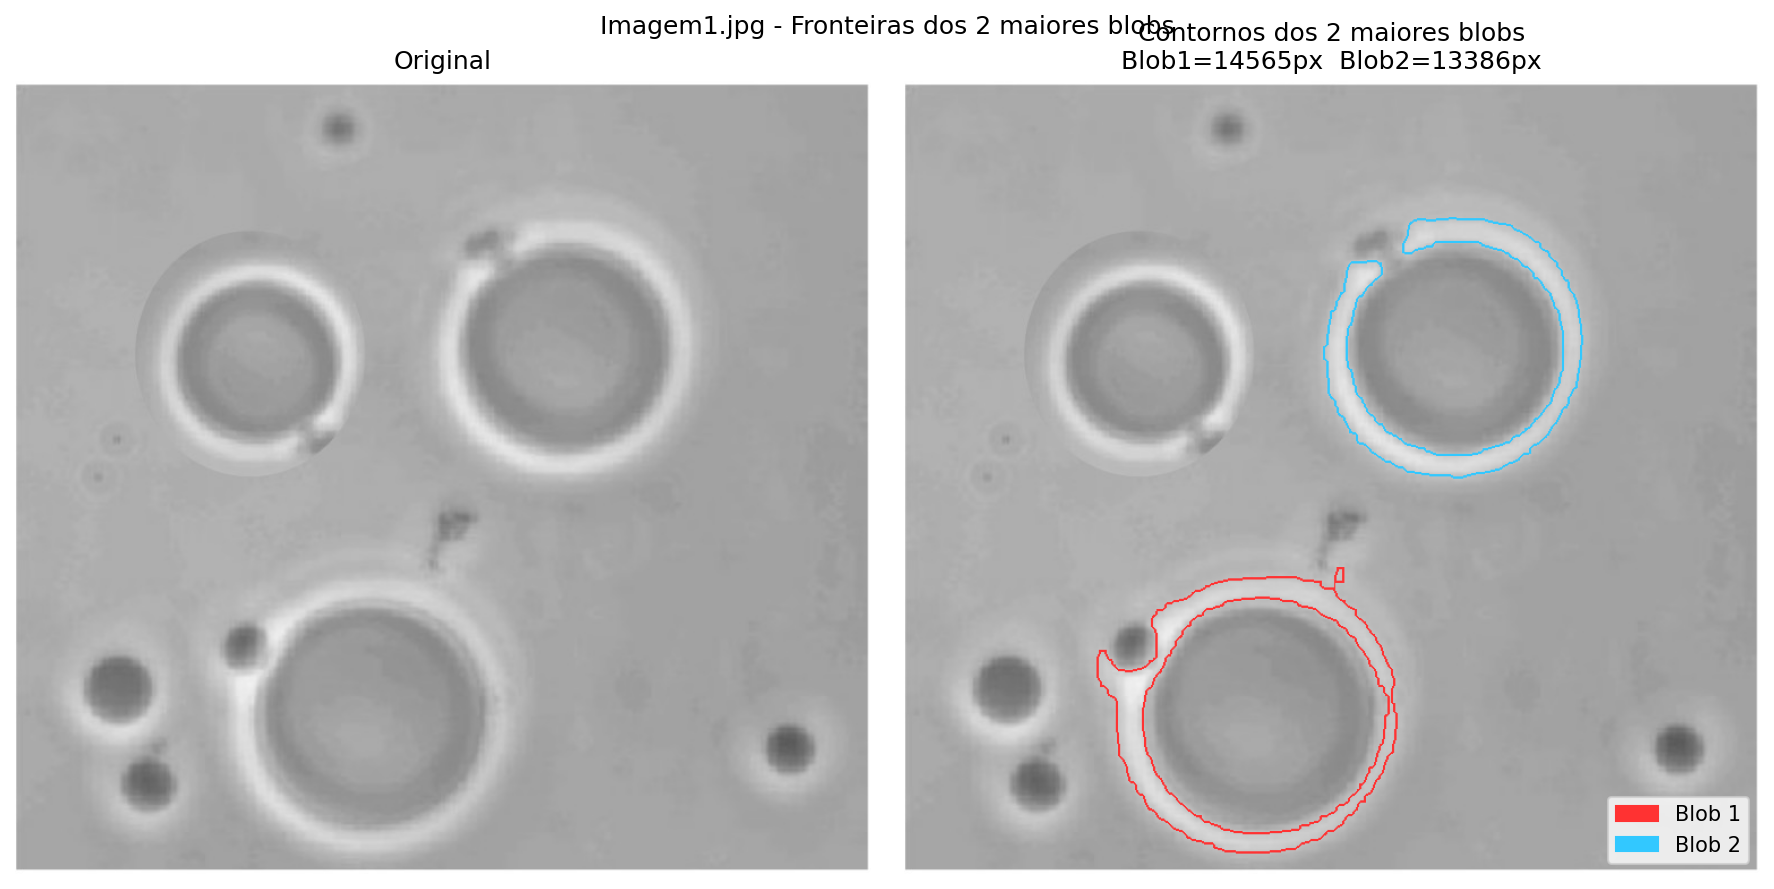
\includegraphics[width=0.85\linewidth]{imgs_result/imagem1_boundary.png}
  \caption{Imagem1.jpg: original e contornos dos dois maiores blobs.}
  \fonte{Elaborado pelo autor (2026).}
\end{figure}

\section{Imagem 2 -- Imagem2.jpg}

\begin{figure}[H]
  \centering
  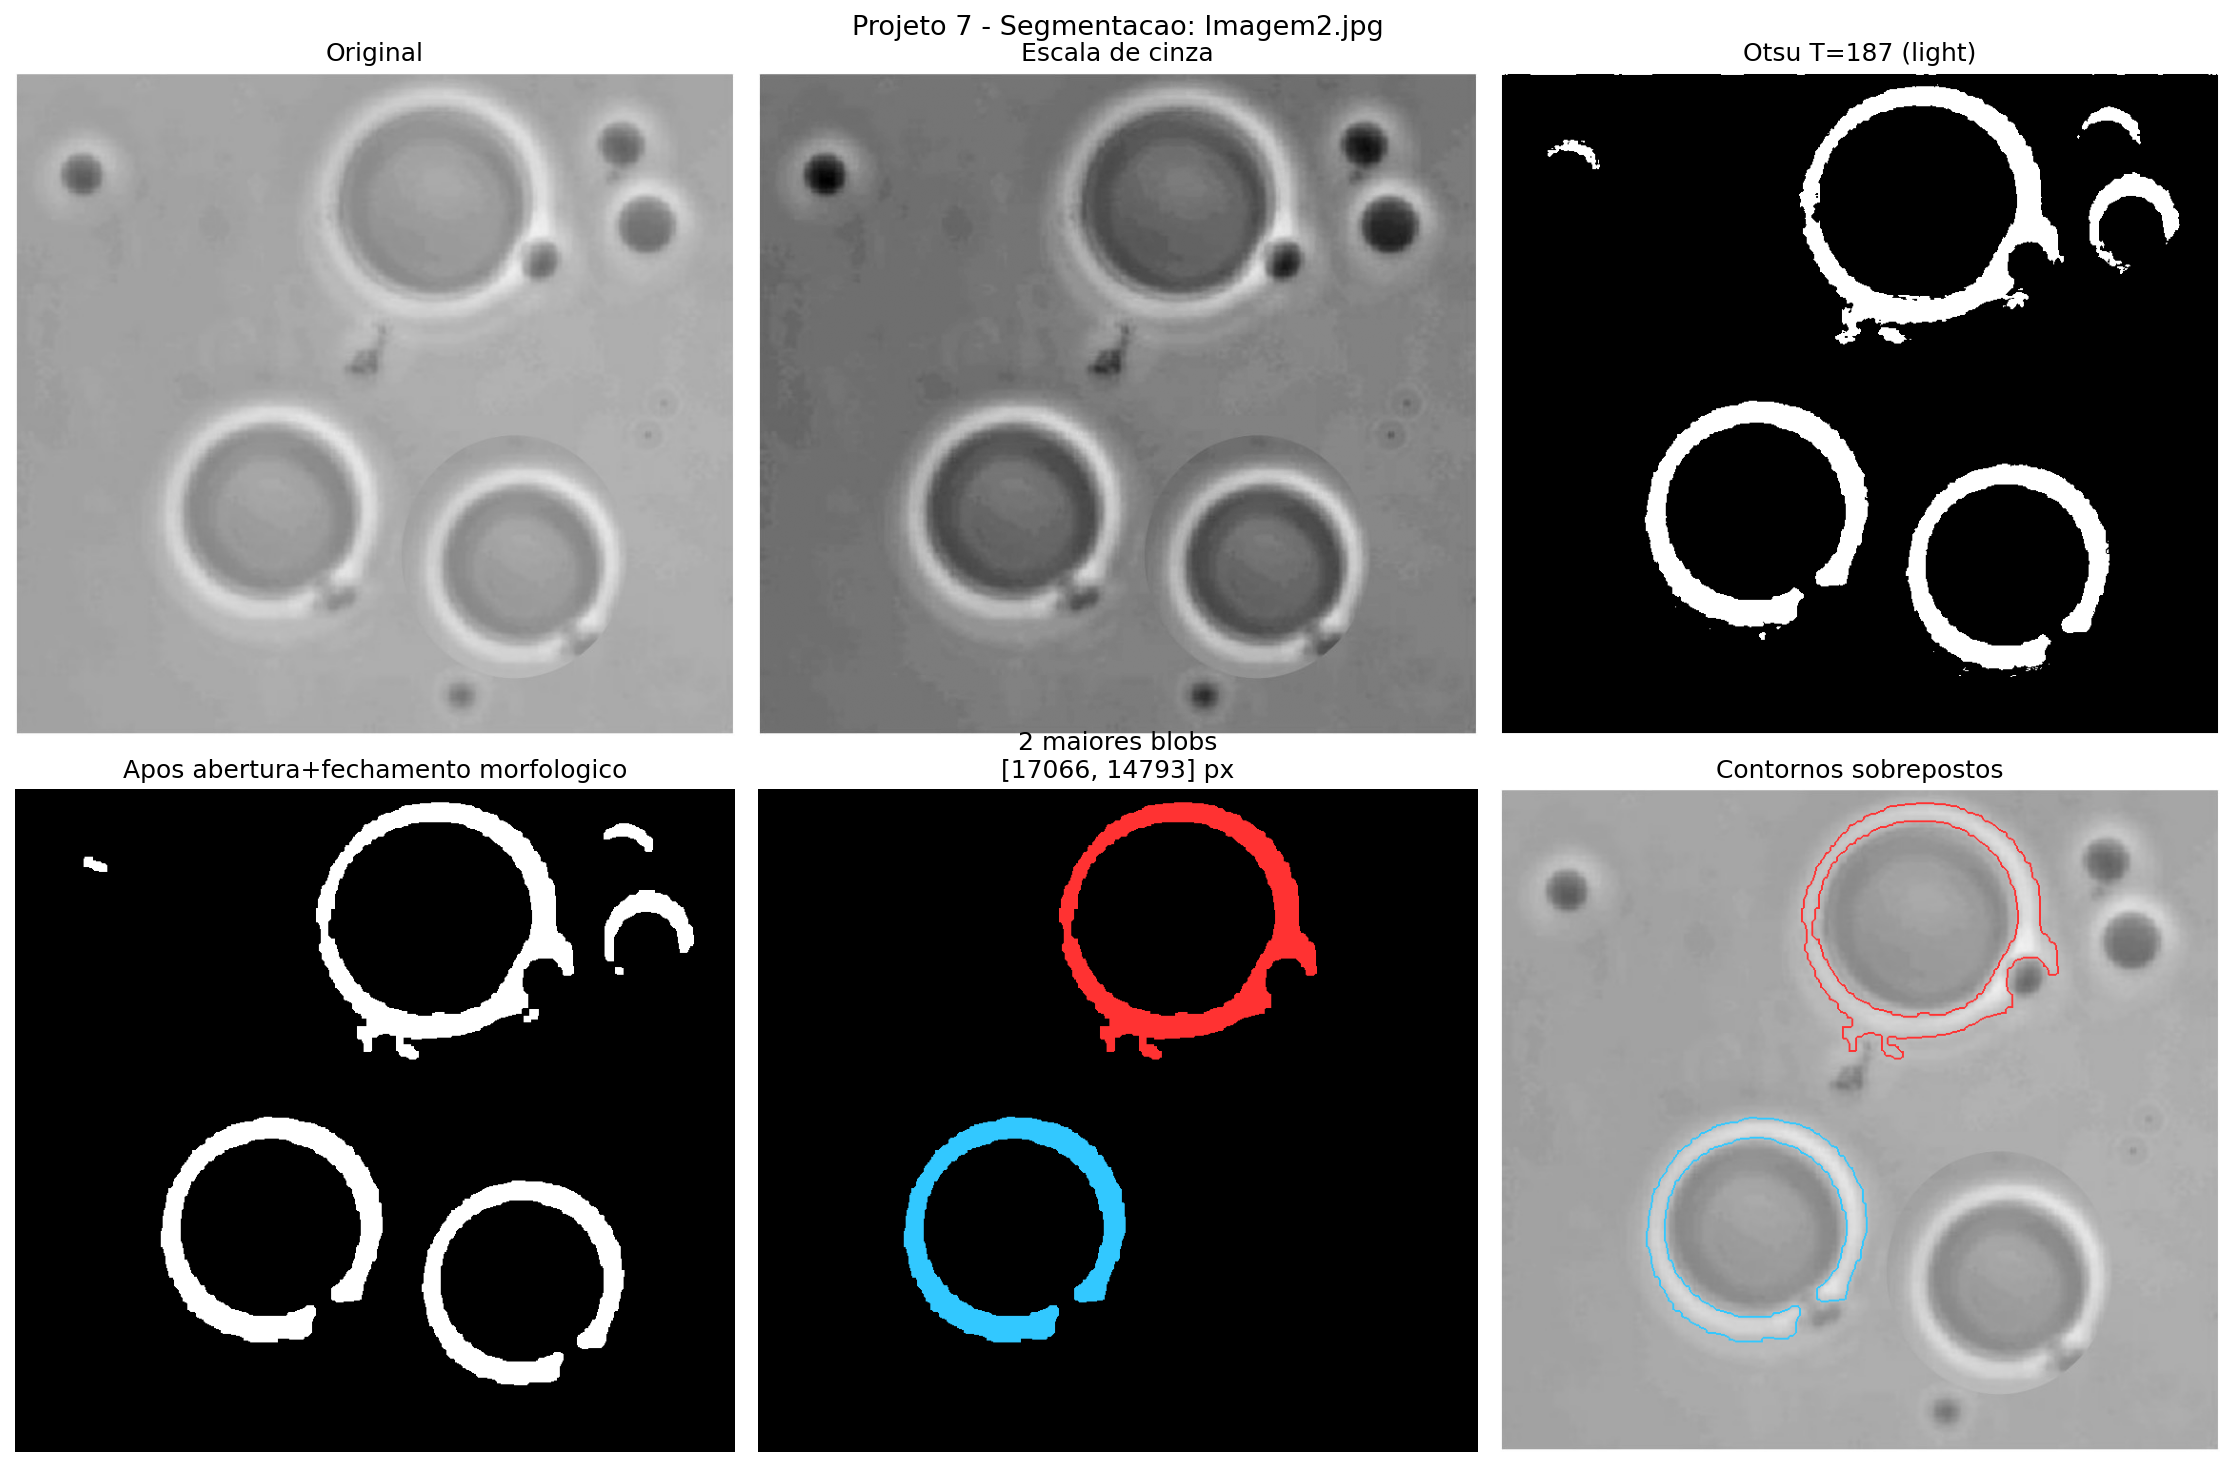
\includegraphics[width=\linewidth]{imgs_result/imagem2_pipeline.png}
  \caption{Pipeline para Imagem2.jpg.
           Limiar $T = 187$; 8~componentes;
           2~maiores: 17.066 e 14.793 pixels.}
  \fonte{Elaborado pelo autor (2026).}
\end{figure}

\begin{figure}[H]
  \centering
  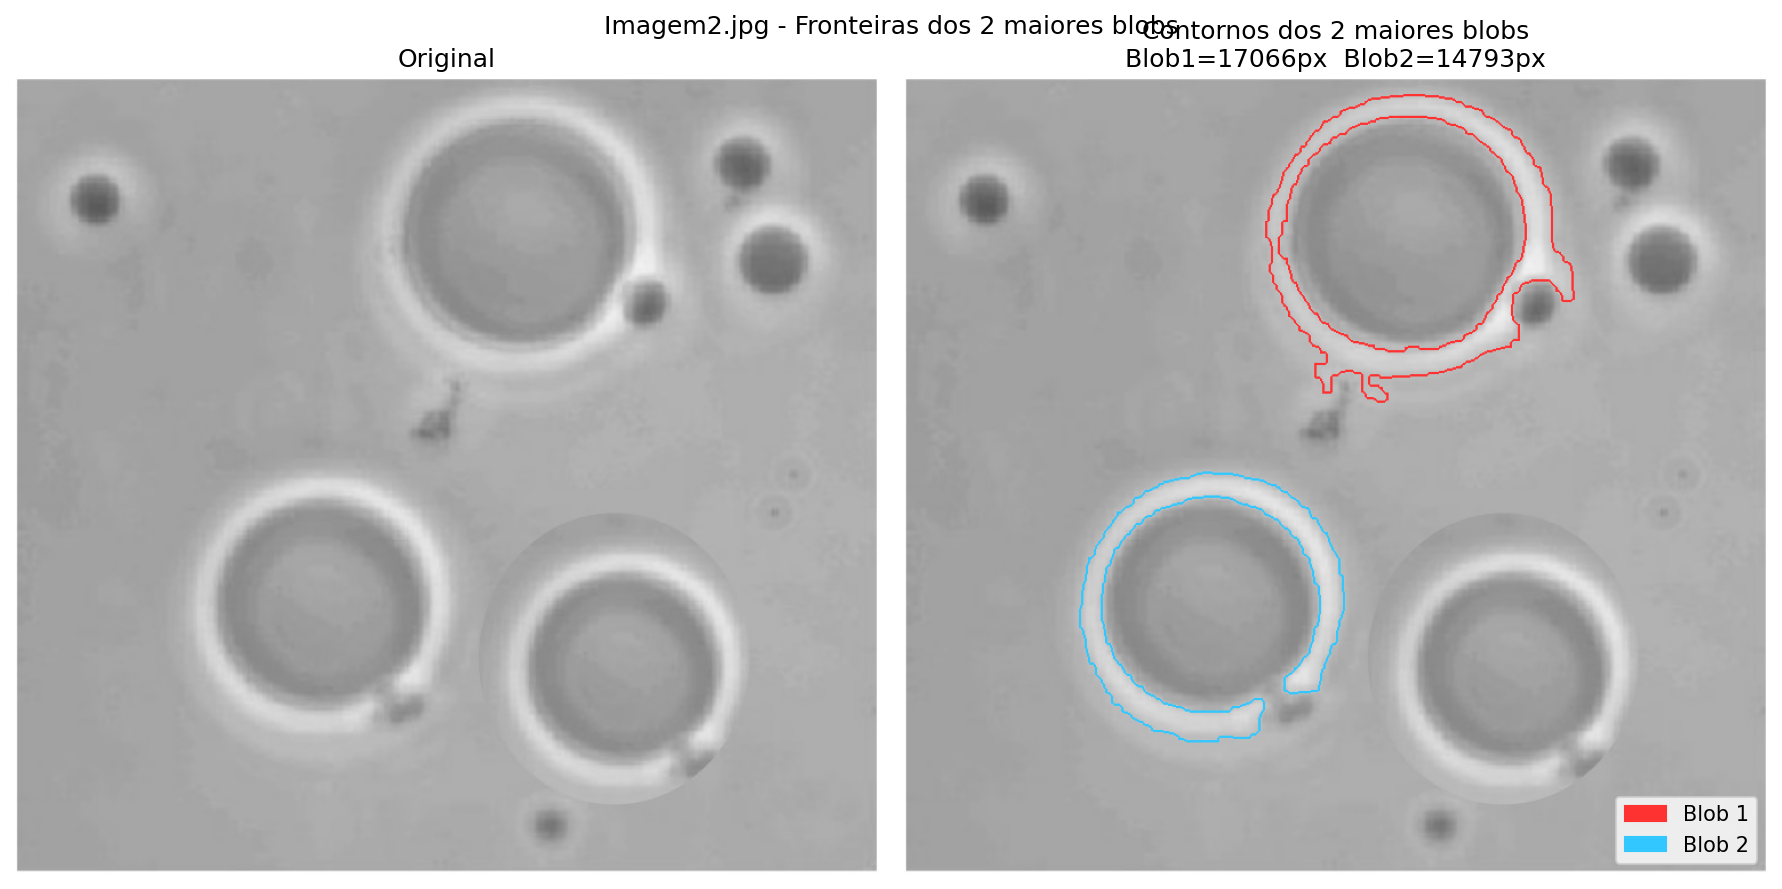
\includegraphics[width=0.85\linewidth]{imgs_result/imagem2_boundary.png}
  \caption{Imagem2.jpg: original e contornos dos dois maiores blobs.}
  \fonte{Elaborado pelo autor (2026).}
\end{figure}

\section{Imagem 3 -- Imagem3.jpg}

\begin{figure}[H]
  \centering
  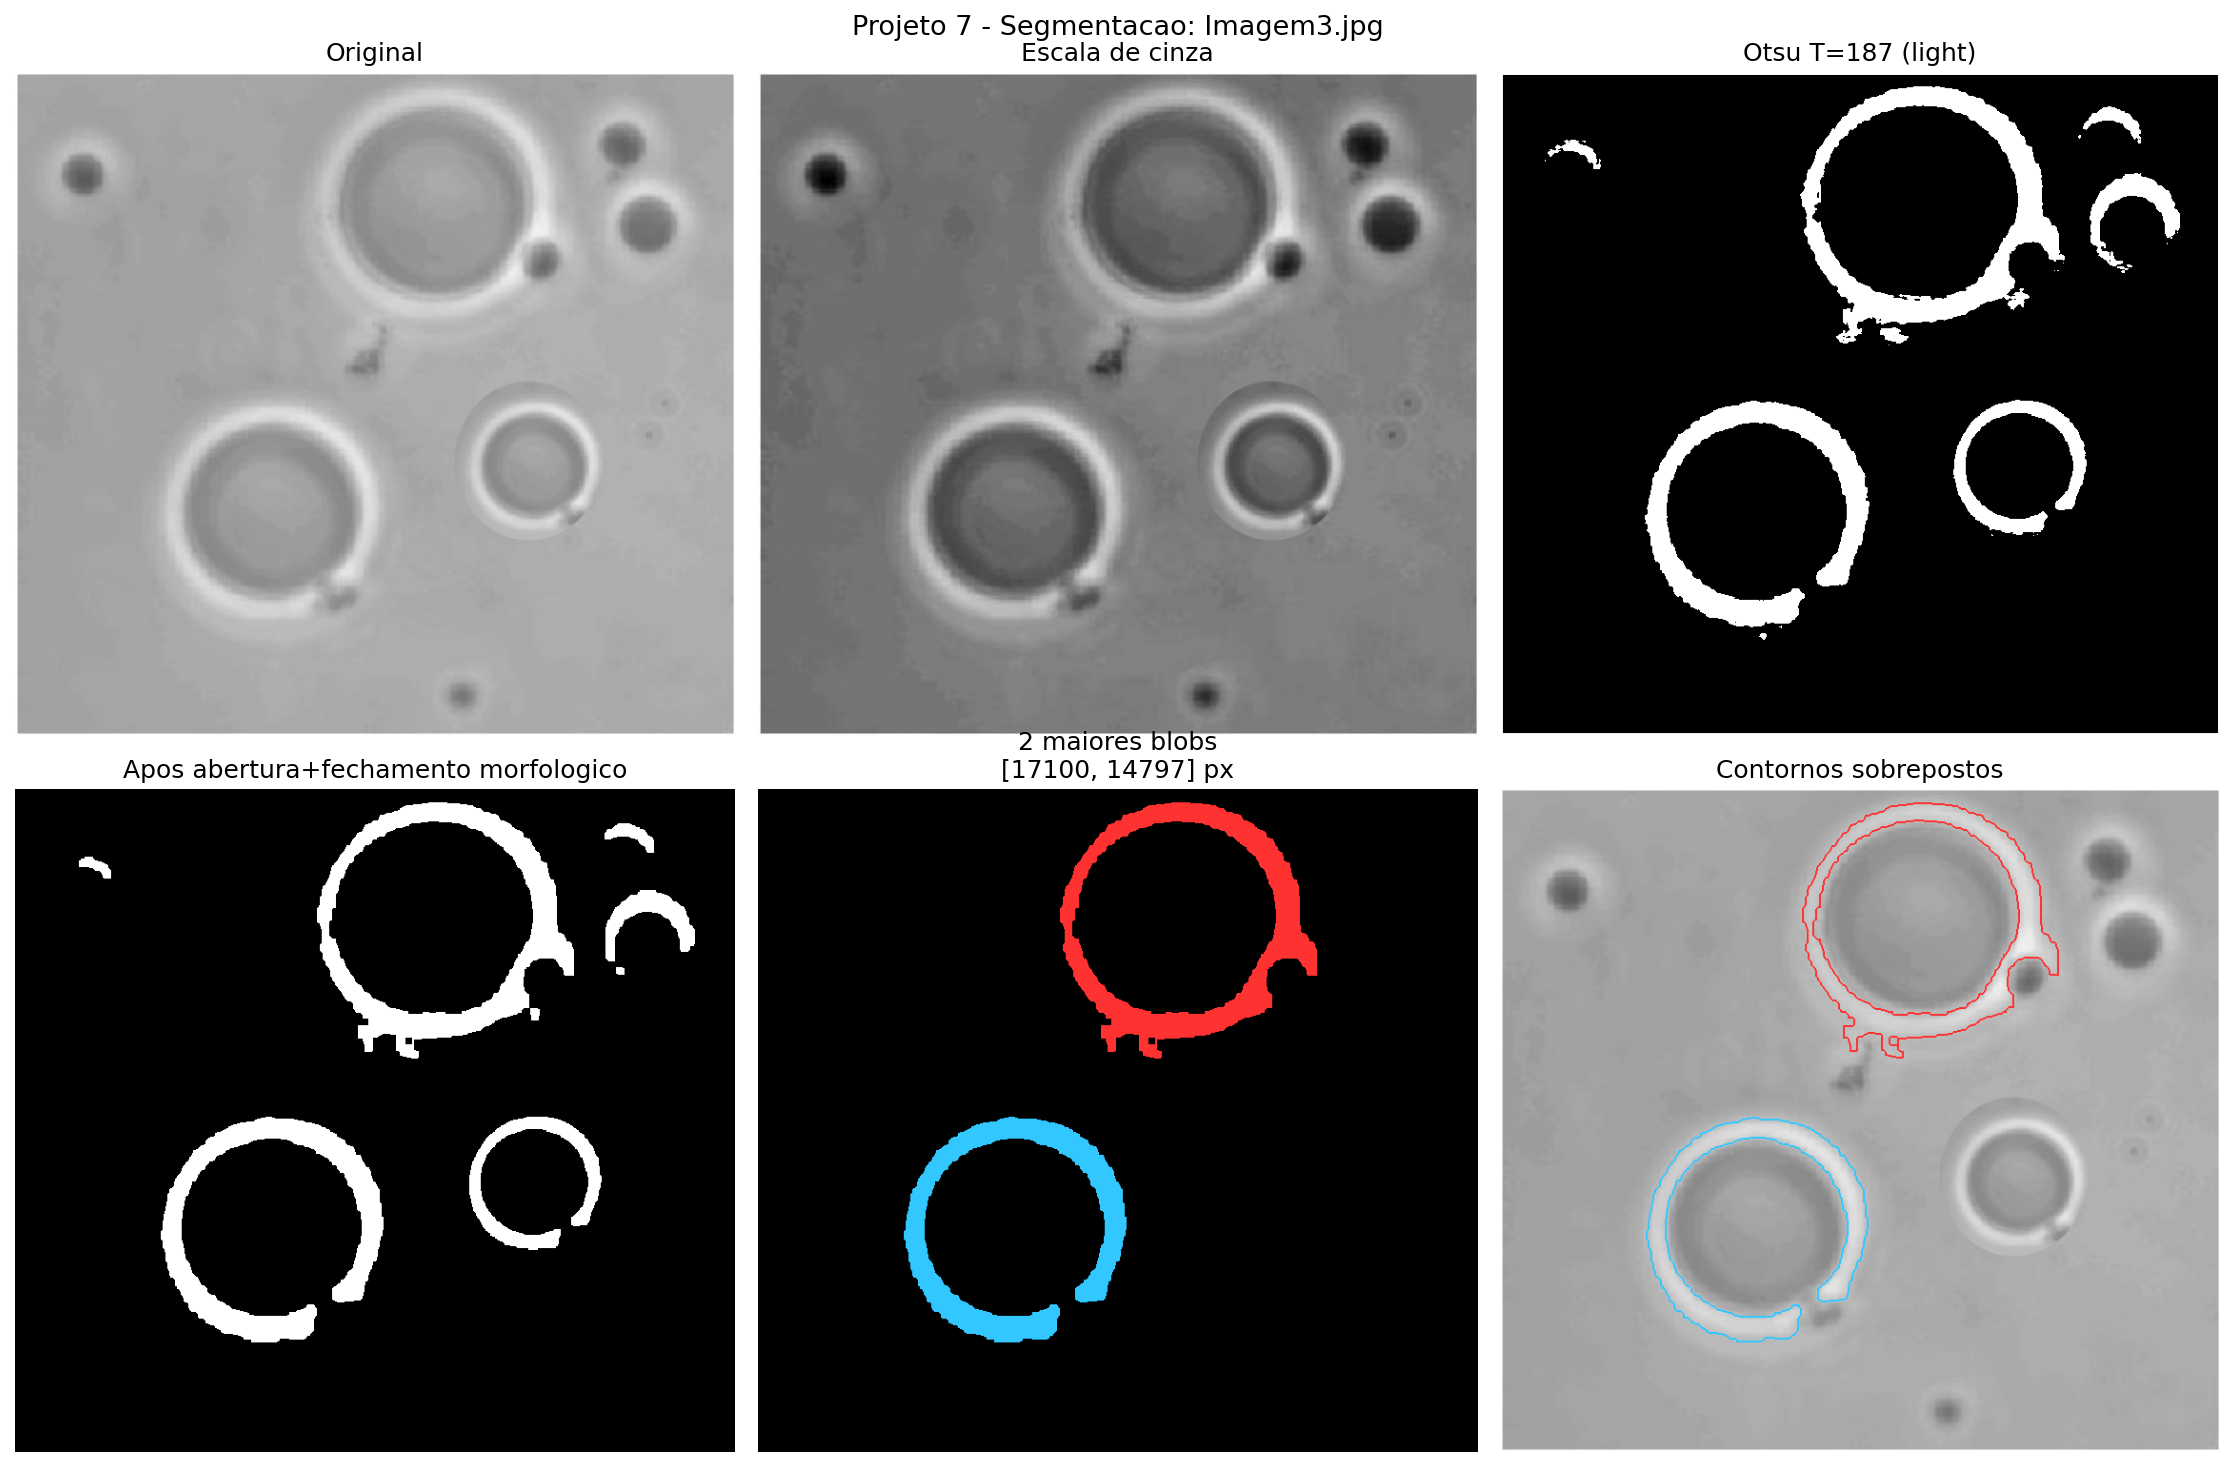
\includegraphics[width=\linewidth]{imgs_result/imagem3_pipeline.png}
  \caption{Pipeline para Imagem3.jpg.
           Limiar $T = 187$; 8~componentes;
           2~maiores: 17.100 e 14.797 pixels.}
  \fonte{Elaborado pelo autor (2026).}
\end{figure}

\begin{figure}[H]
  \centering
  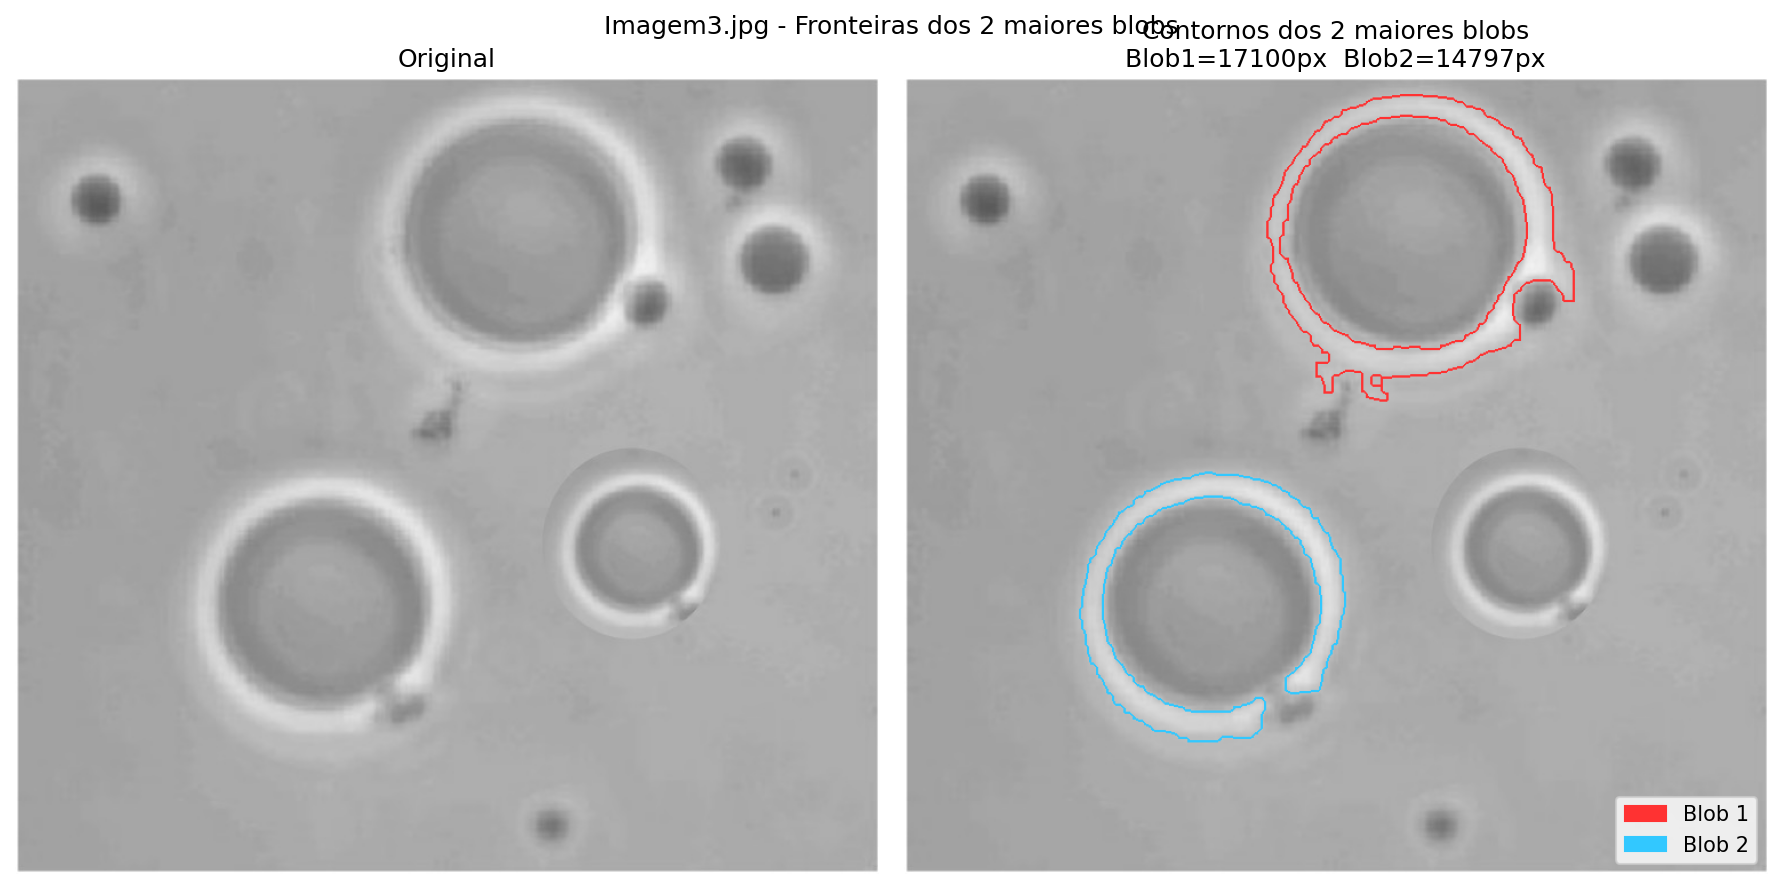
\includegraphics[width=0.85\linewidth]{imgs_result/imagem3_boundary.png}
  \caption{Imagem3.jpg: original e contornos dos dois maiores blobs.}
  \fonte{Elaborado pelo autor (2026).}
\end{figure}

\section{Tabela Comparativa}

\begin{table}[H]
  \centering
  \caption{Resultados quantitativos por imagem.}
  \label{tab:results}
  \begin{tabular}{lcccccc}
    \toprule
    Imagem & Limiar $T$ & Componentes & \multicolumn{2}{c}{\'Area (px)} \\
           &            &             & Blob 1 & Blob 2 \\
    \midrule
    Imagem1.jpg & 190 & 6 & 14.565 & 13.386 \\
    Imagem2.jpg & 187 & 8 & 17.066 & 14.793 \\
    Imagem3.jpg & 187 & 8 & 17.100 & 14.797 \\
    \bottomrule
  \end{tabular}
  \fonte{Elaborado pelo autor (2026).}
\end{table}

%% ----------------------------------------------------------------
\chapter{Conclus\~ao}
%% ----------------------------------------------------------------

O pipeline proposto segmentou com sucesso os dois maiores blobs nas
tr\^es imagens fornecidas.
Os principais resultados s\~ao:

\begin{enumerate}
  \item A limiariza\c{c}\~ao de Otsu determinou automaticamente limiares
        entre 187 e 190, adequados para separar os blobs do fundo em
        todas as imagens;
  \item A limpeza morfol\'ogica (abertura + fechamento com elemento disco
        de raio 3) reduziu o ru\'ido sem comprometer os blobs principais;
  \item O m\'etodo de componentes conectados identificou entre 6 e
        8 regi\~oes por imagem; os dois maiores componentes apresentam
        \'areas entre 13.386 e 17.100 pixels;
  \item A extra\c{c}\~ao de fronteira por diferen\c{c}a morfol\'ogica
        gerou contornos n\'itidos de $\approx$2 pixels de espessura,
        adequados para visualiza\c{c}\~ao sobre a imagem original.
\end{enumerate}

O m\'etodo \'e gen\'erico e parametriz\'avel: o elemento estruturante
e o n\'umero de blobs desejado podem ser ajustados para outras
aplica\c{c}\~oes de segmenta\c{c}\~ao.

\postextual
\bibliography{referencias_project9}

\end{document}
